\documentclass[12pt]{article}
\usepackage{amsmath,amssymb,amsthm}
\usepackage{enumerate,enumitem}
\usepackage{graphicx}
\usepackage{geometry}
\usepackage[dvipsnames]{xcolor}
\usepackage{mathtools}
\usepackage[cm]{fullpage}
\usepackage[english,ukrainian]{babel}
\usepackage[T1,T2A]{fontenc}
\usepackage[utf8]{inputenc}
\usepackage{titlesec}

\usepackage{multirow}
\usepackage{mathtools}
\usepackage{upgreek}

% Extra packages for the demo:
\usepackage{booktabs}
\usepackage{colortbl}
\usepackage{ragged2e}
\usepackage{schemabloc}
\usepackage{commath}
\usepackage{physics}
\usepackage{array}
\usepackage{wrapfig}

\newcolumntype{B}{>{\bfseries}l<}
%~~~~~~~~~~~~~~~~~~~~~~~~~~~~~~~~~~~~~~~~~~~~~~~~~~~~~~~~~~~~~~~~~~~~~~~~~~~~~~
\renewcommand{\d}{\dif}

\parindent 0in

\usepackage{multicol}
\usepackage{setspace}
\setenumerate{nosep, label=\bfseries\alph*.}
\renewcommand{\theenumi}{\alph{enumi}}

%%%%%%%%%%%%%%%%%%%%%%%%%%%%%%%%%%%%%%%%%%%%%%%%%%%%%%%%%%%%
%%%%%%%%%%%%%%%%% ADJUST THESE VALUES %%%%%%%%%%%%%%%%%%%%%%
%%%%%%%%%%%%%%%%%%%%%%%%%%%%%%%%%%%%%%%%%%%%%%%%%%%%%%%%%%%%
\newcommand{\hw}{0}            %% ASSIGNMENT NUMBER %%%%%%%%
\newcommand{\group}{ФБ,ФЕ}        %% GROUP NUMBER %%%%%%%%%%%%%
\newcommand{\coursename}{Фізика}  %% COURSE NAME %%%%%%%%%%%%%%
\newcommand{\term}{1 семестр}
\newcommand{\theme}{Вступ}
%%%%%%%%%%%%%%%%%%%%%%%%%%%%%%%%%%%%%%%%%%%%%%%%%%%%%%%%%%%%

\newtheorem{theorem}{Теорема}
\newcounter{problems}

\newenvironment{problem}[1][]
{\begin{trivlist}\item[\hskip \labelsep {\bfseries #1}\hskip \labelsep {\bfseries \thesection.\arabic{problems}.}]}
{\addtocounter{problems}{1}
\end{trivlist}}

\titleformat{\section}
{\color{WildStrawberry}\normalfont\Large\bfseries}
{\color{WildStrawberry}Заняття \thesection \setcounter{problems}{1}}{1em}{}

\usepackage{floatrow}
\usepackage{subfigure}
\usepackage{graphicx,wrapfig}
\floatsetup[table]{capposition=top}
\floatsetup[wrapfigure]{capposition=bottom}
%\floatsetup[figure]{capposition=beside,%
%                    capbesideposition={right,bottom},%
%                    capbesidewidth=0.3\textwidth,%
%                    capbesidesep=quad% разделитель между картинкой и подписью
%}
\usepackage{amsmath}

\begin{document}
\everymath{\displaystyle}

\thispagestyle{empty}
\pagestyle{empty}

%\textbf{Групи \group}\hfill\textbf{\coursename, \term}\\ 

\newcommand{\ans}{\textit{\textbf{Відповідь: }}}
\newcommand{\nb}{\textit{\textbf{Вказівка. }}}

\newcommand{\preambula}[4]{

\begin{minipage}[h]{0.2\linewidth}
	\vspace{-1.6cm}
	\textbf{Дано:}
	
    #1
    
	\hrulefill
	#2
	\end{minipage}
	\hspace{-0.3cm}
	\vline
	\hfill
	\hspace{-0.6cm}
	\begin{minipage}[h]{0.45\linewidth}
	#3
    \end{minipage}
    \begin{minipage}[h]{0.22\linewidth}
    %\vspace{-5ex}
    \includegraphics[width=\linewidth]{#4}
    %\hspace{4ex}
    %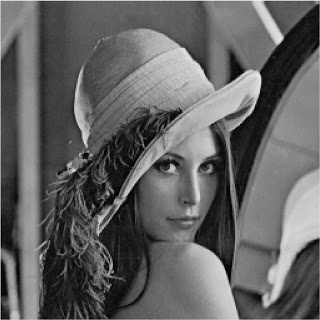
\includegraphics[width=\linewidth]{image}
    \label{ris}
	\end{minipage}
}

\newcommand{\given}{}
\newcommand{\question}{}
\newcommand{\innertext}{}
\newcommand{\imageone}{image}

\newcommand{\genpreambula}{
\preambula{\given}{\question}{\innertext}{\imageone}
}


%%%%%%%%%%%%%%%%%%%%%%%%%%%%%%%%%%%%%%%%%%%%%%%%%%%%%%%%%%%%
%%%%%%%%%%%%%%%%%%%% BEGIN PROBLEMS %%%%%%%%%%%%%%%%%%%%%%%%
%%%%%%%%%%%%%%%%%%%%%%%%%%%%%%%%%%%%%%%%%%%%%%%%%%%%%%%%%%%%
%\tableofcontents
%\newpage

%\input{00-1.tex} 
%\input{00-2.tex} 
%\input{00-3.tex} 
%%%%%%%%%%%%%%%%%%%%%%%

%\input{01.tex} % Е, потенціал. 12-19.02.19
%%%%%%%%%%%%%%%%%%%%%%%
%\setcounter{section}{5}

\section{Інтегрування полів: потік векторного поля. Теорема Гауса для електричного поля}
%%%%%%%%%%%%%%%%%%%%%%%%%%%%%%%%%%%%%%%
\begin{problem}{1}
Знайти напруженість поля рівномірно зарядженої площини з поверхневою густиною заряду~$\sigma$.
\end{problem}

\begin{problem}{2}
Знайти напруженість поля двох паралельних площин. Відома поверхнева густина заряду~$\sigma$.
\end{problem}

\begin{problem}{3}
Знайти напруженість поля рівномірно зарядженої сферичної поверхні. Радіус поверхні $R$, заряд $-q$.
\end{problem}

\begin{problem}{4}
Визначити потік $\Phi$ вектора напруженості електричного поля $Е$ крізь бічну поверхню конуса, висота якого $h = 20$~см і радіус основи $r = 10$~см. На осі конуса на однакових відстанях від вершини й центра основи розміщений заряд $q = 1$~мкКл. Конус міститься у вакуумі.
\end{problem}

\begin{problem}{5}
У центрі куба міститься точковий заряд $q$. Чому дорівнює потік $\Phi$ вектора напруженості $Е$: а) крізь повну поверхню куба; б) крізь одну з його граней?
\end{problem}

\textbf{Завдання для самостійної роботи}

\begin{problem}{6}
Обчислити потік $\Phi$ вектора напруженості електричного поля $Е$ крізь бічну поверхню прямого кругового циліндра, висота якого $h = 20$~см, а радіус основи $r = 10$~см. Точковий заряд $q= 0,3$~мкКл міститься: а) на осі циліндра на середині висоти; б) у центрі основи.
\end{problem}

\begin{problem}{7}
Два нескінченних тонкостінних коаксіальних циліндри радіусів $R_1 = 5$~см і $R_2 = 10$~см рівномірно заряджені з поверхневими густинами зарядів $\sigma_1= 10$~нКл/м$^2$ і $\sigma_2= -3$~нКл/м$^2$. Простір між циліндрами заповнений повітрям.
Визначити модуль $Е$ напруженості поля в точках, що містяться на відстанях $r_1 = 2$~см, $r_2 =6$~см, $r_3 = 15$~см від осі циліндрів.
\end{problem}

\begin{problem}{8}
Усередині однорідно зарядженої кулі з об'ємною густиною заряду $\sigma$ міститься сферична порожнина, центр якої зміщений відносно центра кулі на відстань $r_0$. Визначити напруженість $Е$~поля всередині порожнини. Якою вона буде при $r_0 = 0$? 

\nb Скористатися принципом суперпозиції полів
позитивно об'ємнo зарядженої кулі і негативно об'ємно зарядженої кулі з радіусом порожнини.
\end{problem} % 26.02.19 
\setcounter{section}{5}

\section{Інтегрування полів: потік векторного поля. Теорема Гауса для електричного поля}
%%%%%%%%%%%%%%%%%%%%%%%%%%%%%%%%%%%%%%%

\hrulefill
\begin{theorem}[Теорема Гауса для електричного поля]
$\oint\limits_S \Vec{E} \cdot \Vec{n} \d S = \frac{Q}{\varepsilon_{0}} = \frac{1}{\varepsilon_{0}} \oint_V \rho \d V$ \\
Потік електричного поля через довільну \textbf{замкнену} поверхню рівний сумарному електричному заряду всередині цієї поверхні, помноженому на $\frac{1}{\varepsilon_{0}}$.
\end{theorem}
\hrulefill

\begin{problem}
Знайти напруженість поля рівномірно зарядженої площини з поверхневою густиною заряду~$\sigma$.
\end{problem}
	
\renewcommand{\given}{}
\renewcommand{\question}{}
\renewcommand{\innertext}{}
\renewcommand{\imageone}{image}

\genpreambula


	
	
%\input{03} % 05.03.19

%\input{04-ir.tex} % 12.03.19
%\input{05-ir.tex} % 19.03.19

%\input{06.tex} %26.03.19 ємність. енергія
%\input{07.tex} %02.04.19 струм - 
%\input{08.tex} 

%\input{09.tex}
%\input{10.tex}
%%%%%%%%%%%%%%%%%%%%%%%
%\input{11.tex}
%\input{12.tex}

\end{document} 